
\documentclass{article}
\usepackage{tikz}
\usepackage{verbatim}


% Parameter
\newcommand{\circdist}{1.2}  % Strecke center zum Mittelpunkt der Kreise
\newcommand{\circrad}{7/4} % radius der Kreise
\newcommand{\circlethickness}{6mm} % Dicke


% Definition der Freifunk Farben

\definecolor{FFgelb}{HTML}{FFB400}  
\definecolor{FFmagenta}{HTML}{DC0067}
\definecolor{FFblau}{HTML}{009EE0}

% Farbwahl über Winkel

\colorlet{20}{FFmagenta}
\colorlet{180}{FFmagenta}

% ====================================================================
%
%         Die 3 verschiedenen Kreise
%
% ====================================================================

\newcommand{\mycircle}[1]{%
  \draw[FFmagenta, double distance=\circlethickness, double=#1]
  (#1:\circdist) circle (\circrad);}
  

\newcommand{\freifunks}[1]{%
  \draw[FFmagenta, double distance=2 mm, double=#1]
  (#1:\circdist) circle (7/5);}
  
\newcommand{\freifunkleft}[1]{%
  \draw[FFmagenta, double distance=2 mm, double=#1]
  (#1:\circdist) 
  circle (7/5);}

% ====================================================================
%
%         Dokumenten-Anfang
%
% ====================================================================

\begin{document}

% ====================================================================
%
%         Linke Seite Streifen
%
% ====================================================================

    \begin{tikzpicture}[overlay,remember picture]
    \node [
      fill=FFblau,% Farbe des Randstreifens
      text=white,% Textfarbe
      font=\normalfont\bfseries,% Einstellungen für die Schrift
      inner xsep=1em, % Abstand des Textes von unten
      % maximale Textbreite = Papierhöhe - 2*Abstand des Textes von unten:
      text width={\dimexpr\paperheight-2em\relax},
      minimum height=15mm,% Breite des Randstreifens
      anchor=north east,
      rotate=90
      ]
      at (current page.north west)
      {fulda.freifunk.net};
  \end{tikzpicture}%

% ====================================================================
%
%         Rechte Seite Streifen
%
% ====================================================================

\begin{tikzpicture}[overlay,remember picture]
    \node [
      fill=FFgelb,% Farbe des Randstreifens
      text=white,% Textfarbe
      font=\normalfont\bfseries,% Einstellungen für die Schrift
      inner xsep=1em, % Abstand des Textes von unten
      % maximale Textbreite = Papierhöhe - 2*Abstand des Textes von unten:
      text width={\dimexpr\paperheight-1em\relax},
      minimum height=25mm,% Breite des Randstreifens
      anchor=north,
      rotate=270
      ]
      at (current page.east){\rotatebox{180}{}};


      % \node[anchor=east, rotate=90] at (current page.east) {};
\end{tikzpicture}

\begin{tikzpicture}[overlay,remember picture]
    \node [
      fill=white,% Farbe des Randstreifens
      text=white,% Textfarbe
      font=\normalfont\bfseries,% Einstellungen für die Schrift
      inner xsep=1em, % Abstand des Textes von unten
      % maximale Textbreite = Papierhöhe - 2*Abstand des Textes von unten:
      text width={\dimexpr\paperheight-1em\relax},
      minimum height=20mm,% Breite des Randstreifens
      anchor=north,
      rotate=270
      ]
      at (current page.east){\rotatebox{180}{}};


      % \node[anchor=east, rotate=90] at (current page.east) {};
\end{tikzpicture}

\begin{tikzpicture}[overlay,remember picture]
    \node [
      fill=FFmagenta,% Farbe des Randstreifens
      text=white,% Textfarbe
      font=\normalfont\bfseries,% Einstellungen für die Schrift
      inner xsep=1em, % Abstand des Textes von unten
      % maximale Textbreite = Papierhöhe - 2*Abstand des Textes von unten:
      text width={\dimexpr\paperheight-1em\relax},
      minimum height=15mm,% Breite des Randstreifens
      anchor=north,
      rotate=270
      ]
      at (current page.east){\rotatebox{180}{Einrichten eines: TP-LINK WDR 4300 v1.0}};


      % \node[anchor=east, rotate=90] at (current page.east) {};
\end{tikzpicture}



% ====================================================================
%
%         Inhalt (Mitte)
%
% ====================================================================


\begin{center}

  % \begin{tikzpicture}
  %   \draw[yellow,line width=1cm] (0,0) circle[radius=2cm];
  % \end{tikzpicture}

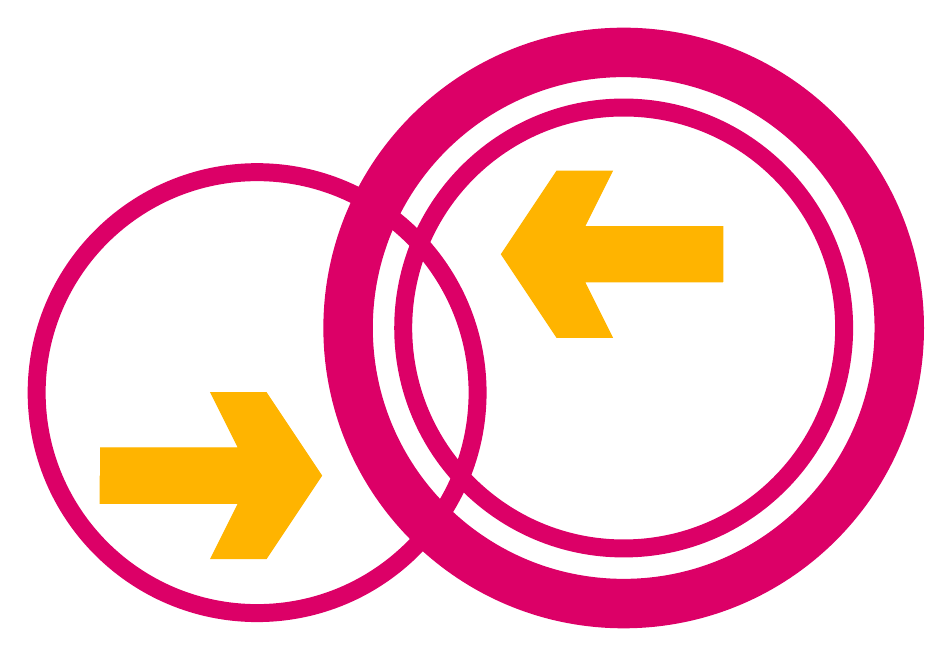
\begin{tikzpicture}[scale=2]

  % draw the circles
%  \foreach \angle in {180,20}
%  {
%    \mycircle{\angle}
%  }
	\freifunkleft{180}
	\mycircle{20}
  \freifunks{20}

%   \filldraw[fill=FFgelb, color=FFgelb]
% (0em,2em) -- (3em,2em) -- (2.5em,1em) -- (3.5em,1em) -- (4.5em,2.5em) %
% -- (3.5em,4em) -- (2.5em,4em) -- (3em,3em) --(0em,3em)
% -- (0em,2em) ;


  \filldraw[fill=FFgelb, color=FFgelb]
(5em,2em) -- (2.5em,2em) -- (3.0em,1em) -- (2em,1em) -- (1em,2.5em) %
-- (2em,4em) -- (3em,4em) -- (2.5em,3em) --(5em,3em)
-- (5em,2em) ;



  \filldraw[fill=FFgelb, color=FFgelb]
(-6.25em,-1.0em) -- (-3.75em,-1.0em) -- (-4.25em,-0.0em) -- (-3.25em,-0.0em) -- (-2.25em,-1.5em) %
-- (-3.25em,-3.0em) -- (-4.25em,-3.0em) -- (-3.75em,-2.0em) --(-6.25em,-2.0em)
-- (-6.25em,-1.5em) ;



\end{tikzpicture}



% Schriftzug Mitte

\huge{fulda.freifunk.net}




\end{center}
\newpage
\Huge{}fulda.freifunk.net
\end{document}